
The compilation of C++ source code appears to be a fairly straightforward process. Let's take a small program, such as a classic hello.cpp application, as follows:

\begin{lstlisting}[style=styleCXX]
// chapter-01/01-hello/hello.cpp

#include <iostream>
int main() {
	std::cout << "Hello World!" << std::endl;
	return 0;
}
\end{lstlisting}

Now, all we need to do to get an executable is to run a single command. We call the compiler with the filename as an argument:

\begin{tcblisting}{commandshell={}}
$ g++ hello.cpp -o a.out
\end{tcblisting}

Our code is correct, so the compiler will silently produce an executable binary file that our machine can understand. We can run it by calling its name:

\begin{tcblisting}{commandshell={}}
$ ./a.out
Hello World!
$
\end{tcblisting}

However, as our projects grow, you will quickly understand that keeping everything in a single file is simply not possible. Clean code practices recommend that files should be kept small and in well-organized structures. The manual compilation of every file can be a tiresome and fragile process. There must be a better way.

\subsubsubsection{1.2.1\hspace{0.2cm}What is CMake?}

Let's say we automate building by writing a script that goes through our project tree and compiles everything. To avoid any unnecessary compilations, our script will detect whether the source has been modified since the last time we ran it (the script). Now, we'd like a convenient way to manage arguments that are passed to the compiler for each file – preferably, we'd like to do that based on configurable criteria. Additionally, our script should know how to link all of the compiled files in a binary or, even better, build whole solutions that can be reused and incorporated as modules in bigger projects.

The more features we will add the higher the chance that we will get to a full-fledged solution. Building software is a very versatile process and can span multiple different aspects:

\begin{itemize}
\item 
Compiling executables and libraries

\item 
Managing dependencies

\item 
Testing

\item 
Installing

\item 
Packaging

\item 
Producing documentation

\item 
Testing some more
\end{itemize}

It would take a very long time to come up with a truly modular and powerful C++ building application that is fit for every purpose. And it did. Bill Hoffman at Kitware implemented the first versions of CMake over 20 years ago. As you might have already guessed, it was very successful. It now has a lot of features and support from the community. Today, CMake is being actively  developed and has become the industry standard for C and C++ programmers.

The problem of building code in an automated way is much older than CMake, so naturally, there are plenty of options out there: Make, Autotools, SCons, Ninja, Premake, and more. But why does CMake have the upper hand?

There are a couple of things about CMake that I find (granted, subjectively) important:

\begin{itemize}
\item 
It stays focused on supporting modern compilers and toolchains.

\item 
CMake is truly cross-platform – it supports building for Windows, Linux, macOS, and Cygwin.

\item 
It generates project files for popular IDEs: Microsoft Visual Studio, Xcode, and Eclipse CDT. Additionally, it is a project model for others such as CLion.

\item 
CMake operates on just the right level of abstraction – it allows you to group files in reusable targets and projects.

\item 
There are tons of projects that are built with CMake and offer an easy way to include them in your project.

\item 
CMake views testing, packaging, and installing as an inherent part of the build process.

\item 
Old, unused features get deprecated to keep CMake lean.
\end{itemize}

CMake provides a unified, streamlined experience across the board. It doesn't matter if you're building your software in an IDE or directly from the command line; what's really important is it takes care of post-build stages as well. Your Continous Integration/Continous Deployment (CI/CD) pipeline can easily use the same CMake configuration and build projects using a single standard even if all of the preceding environments differ.

\subsubsubsection{1.2.2\hspace{0.2cm}How does it work?}

You might be under the impression that CMake is a tool that reads source code on one end and produces binaries on the other – while that's true in principle, it's not the full picture.

CMake can't build anything on its own – it relies on other tools in the system to perform the actual compilation, linking, and other tasks. You can think of it as the orchestrator of your building process: it knows what steps need to be done, what the end goal is, and how to find the right workers and materials for the job.

This process has three stages:

\begin{itemize}
\item 
Configuration

\item 
Generation

\item 
Building
\end{itemize}

\hspace*{\fill} \\ %插入空行
\noindent
\textbf{The configuration stage}

This stage is about reading project details stored in a directory, called the source tree, and preparing an output directory or build tree for the generation stage. CMake starts by creating an empty build tree and collecting all of the details about the environment it is working in, for example, the architecture, the available compilers, the linkers, and the archivers. Additionally, it checks whether a simple test program can be compiled correctly.

Next, the CMakeLists.txt project configuration file is parsed and executed (yes, CMake projects are configured with CMake's coding language). This file is the bare minimum of a CMake project (source files can be added later). It tells CMake about the project structure, its targets, and its dependencies (libraries and other CMake packages). During this process, CMake stores collected information in the build tree such as system details, project configurations, logs, and temp files, which are used for the next step. Specifically, a CMakeCache.txt file is created to store more stable variables (such as paths to compilers and other tools) and save time during the next configuration.

\hspace*{\fill} \\ %插入空行
\noindent
\textbf{The generation stage}

After reading the project configuration, CMake will generate a buildsystem for the exact environment it is working in. Buildsystems are simply cut-to-size configuration files for other build tools (for example, Makefiles for GNU Make or Ninja and IDE project files for Visual Studio). During this stage, CMake can still apply some final touches to the build configuration by evaluating generator expressions.

\begin{tcolorbox}[colback=blue!5!white,colframe=blue!75!black,title=Note]
The generation stage is executed automatically after the configuration stage. For this reason, this book and other resources often refer to both of these stages when mentioning "configuration" or "generation" of a buildsystem. To explicitly run just the configuration stage, you can use the cmake-gui utility.
\end{tcolorbox}

\hspace*{\fill} \\ %插入空行
\noindent
\textbf{The building stage}

To produce the final artifacts specified in our project, we have to run the appropriate build tool. This can be invoked directly, through an IDE, or using the CMake command. In turn, these build tools will execute steps to produce targets with compilers, linkers, static and dynamic analysis tools, test frameworks, reporting tools, and anything else you can think of.

The beauty of this solution lies in the ability to produce buildsystems on demand for every platform with a single configuration (that is, the same project files):

\begin{center}
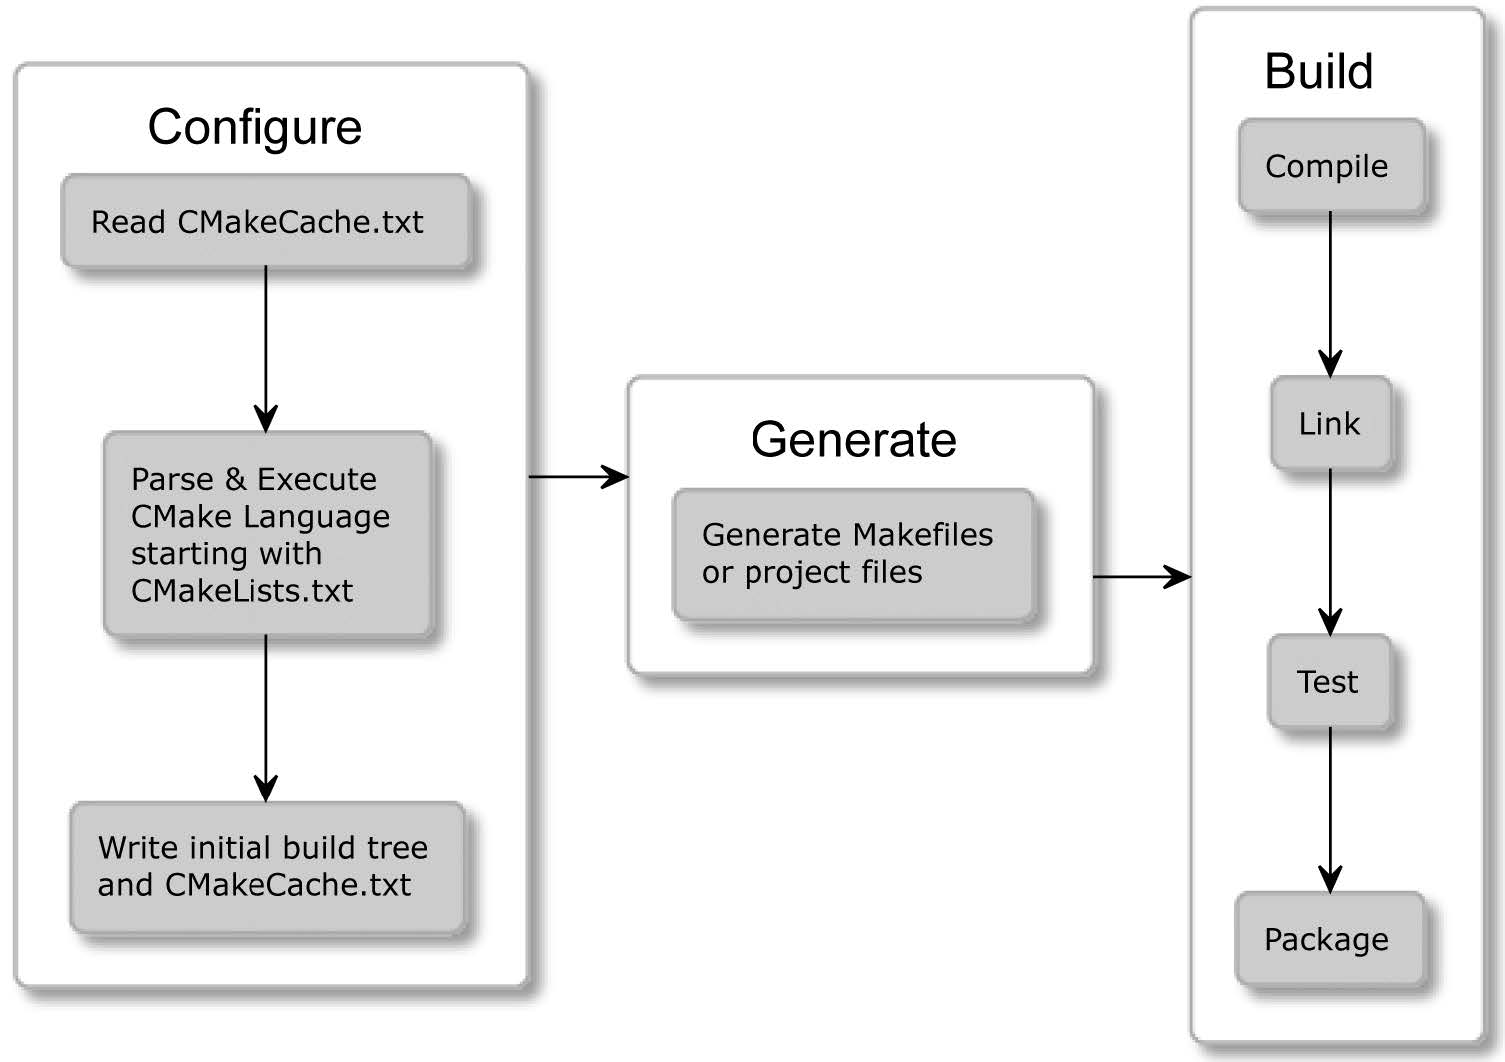
\includegraphics[width=0.9\textwidth]{content/1/chapter1/images/1.jpg}\\
Figure 1.1 – The stages of CMake
\end{center}

Do you remember our hello.cpp application from the Understanding the basics section? CMake makes it really easy for you to build it. All we need is the following CMakeLists.txt file next to our source and two simple commands, cmake -B buildtree and cmake --build buildtree, as follows:

\begin{lstlisting}[style=styleCMake]
# chapter01/01-hello/CMakeLists.txt: Hello world in the CMake language
	
cmake_minimum_required(VERSION 3.20
project(Hello)
add_executable(Hello hello.cpp)
\end{lstlisting}

Here is the output from the Dockerized Linux system (note that we'll discuss Docker in the Installing CMake on different platforms section):

\begin{tcblisting}{commandshell={}}
root@5f81fe44c9bd:/root/examples/chapter01/01-hello# cmake
-B buildtree.
-- The C compiler identification is GNU 9.3.0
-- The CXX compiler identification is GNU 9.3.0
-- Check for working C compiler: /usr/bin/cc
-- Check for working C compiler: /usr/bin/cc -- works
-- Detecting C compiler ABI info
-- Detecting C compiler ABI info - done
-- Detecting C compile features
-- Detecting C compile features - done
-- Check for working CXX compiler: /usr/bin/c++
-- Check for working CXX compiler: /usr/bin/c++ -- works
-- Detecting CXX compiler ABI info
-- Detecting CXX compiler ABI info - done
-- Detecting CXX compile features
-- Detecting CXX compile features - done
-- Configuring done
-- Generating done
-- Build files have been written to: /root/examples/
chapter01/01-hello/buildtree
root@5f81fe44c9bd:/root/examples/chapter01/01-hello# cmake
--build buildtree/
Scanning dependencies of target Hello
[ 50%] Building CXX object CMakeFiles/Hello.dir/hello.cpp.o
[100%] Linking CXX executable Hello
[100%] Built target Hello
\end{tcblisting}

All that's left is to run it:

\begin{tcblisting}{commandshell={}}
root@68c249f65ce2:~# ./buildtree/Hello
Hello World!
\end{tcblisting}

Here, we have generated a buildsystem that is stored in the buildtree directory. Following this, we executed the build stage and produced a final binary that we were able to run.

Now you know what the end result looks like, I'm sure you will be full of questions: what are the prerequisites to this process? What do these commands mean? Why do we need two of them? How do I write my own project files? Do not worry – these questions will be answered in the following sections.

\begin{tcolorbox}[colback=blue!5!white,colframe=blue!75!black,title=Getting Help]
This book will provide you with the most important information that is relevant to the current version of CMake (at the time of writing, this is 3.20). To provide you with the best advice, I have explicitly avoided any deprecated and no longer recommended features. I highly recommend using, at the very least, version 3.15, which is considered "the Modern CMake." If you require more information, you can find the latest, complete documentation online at \url{https://cmake.org/cmake/help/}.
\end{tcolorbox}



















